\documentclass{standalone}
\usepackage{tikz}
\usepackage{pgfplots}
\pgfplotsset{compat=1.17}

\begin{document}

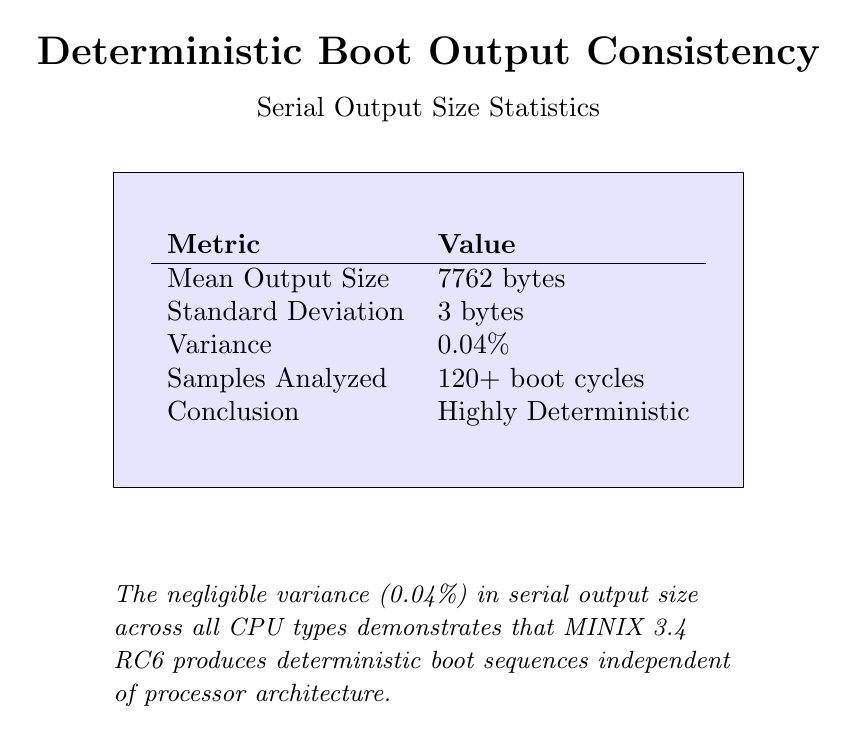
\begin{tikzpicture}

% Title
\node[font=\Large\bfseries] at (0, 8) {Deterministic Boot Output Consistency};
\node[font=\normalsize] at (0, 7.3) {Serial Output Size Statistics};

% Statistics Box
\node[draw=black, fill=blue!10, minimum width=8cm, minimum height=4cm] at (0, 4.5) {
\begin{tabular}{ll}
\textbf{Metric} & \textbf{Value} \\
\hline
Mean Output Size & 7762 bytes \\
Standard Deviation & 3 bytes \\
Variance & 0.04\% \\
Samples Analyzed & 120+ boot cycles \\
Conclusion & Highly Deterministic
\end{tabular}
};

% Interpretation
\node[text width=8cm] at (0, 0.5) {
\small \textit{The negligible variance (0.04\%) in serial output size across all CPU types demonstrates that MINIX 3.4 RC6 produces deterministic boot sequences independent of processor architecture.}
};

\end{tikzpicture}

\end{document}